\section{Introduction}
Autonomous mobile robots (AMRs), including autonomous vehicles \cite{waymo,tesla_robotaxi}, platform AMRs \cite{abb_flexley_mover}, towing AMRs \cite{abb_towing_amrs}, and Goods-to-Person AMRs \cite{abb_goods_to_person}, must operate in complex, unconstrained environments such as public roads, warehouses, semiconductor cleanrooms, and hospital service wings. Although these AMRs often work collaboratively regardless of their specific task, they are routinely confined to narrow hallways, single-lane passages, or one-way roads where two robots cannot pass side by side \cite{fragapane2021planning,xiao2022barn}. When two robots meet head-on in such an aisle, as illustrated in Fig.~\ref{fig:narrow_corridor_examples}, slowing down or swerving laterally is physically insufficient to resolve the conflict. Instead, at least one robot must yield, reversing into an intermediate pull-in bay or retreating entirely from the corridor, typically at a reduced speed limit and under degraded rear sensing. 

These interactions typically require conflict resolution through multi-agent negotiation. Existing paradigms fall into two categories, namely, decentralized local collision-avoidance controllers and centralized coordination schemes. Decentralized controllers, based on velocity obstacles \cite{vandenberg2011orca} or control barrier functions (CBFs) \cite{wang2017safety,grover2023before}, require no inter-robot messaging but reliably fall into symmetric deadlocks in narrow head-on configurations \cite{grover2023before,dergachev2021distributed,zheng2023deadlock,chandra2025deadlock}. 
Such deadlocks are already evident across commercial deployments \cite{stuff_robotaxi_standoff, king_waymo_standoff, dnistran_cruise_gridlock, nyt_waymo_honking}, where mutual hesitation leaves AMRs stranded on public roads. Beyond causing localized traffic disruptions, these highly visible failures severely undermine public trust and amplify skepticism about the readiness of autonomous fleets. Centralized methods, by contrast, including multi-agent path finding (MAPF) \cite{sharon2015cbs,stern2019mapf,okumura2022pibt}, zone-control locks \cite{fanti2002event}, and industrial fleet managers such as Open-RMF \cite{openrmf} and VDA~5050 \cite{vda5050}, prevent conflicts globally but assume common map ownership, reliable infrastructure connectivity, and a single coordinating authority. These assumptions are violated in ad hoc deployments, radio-shadowed aisles, and multi-vendor facilities \cite{gautier2022negotiated,gielis2022critical}. 

\begin{figure*}[!t]
  \centering
  \subfloat[Single-track public road \cite{robson2013singletrack}.]{%
    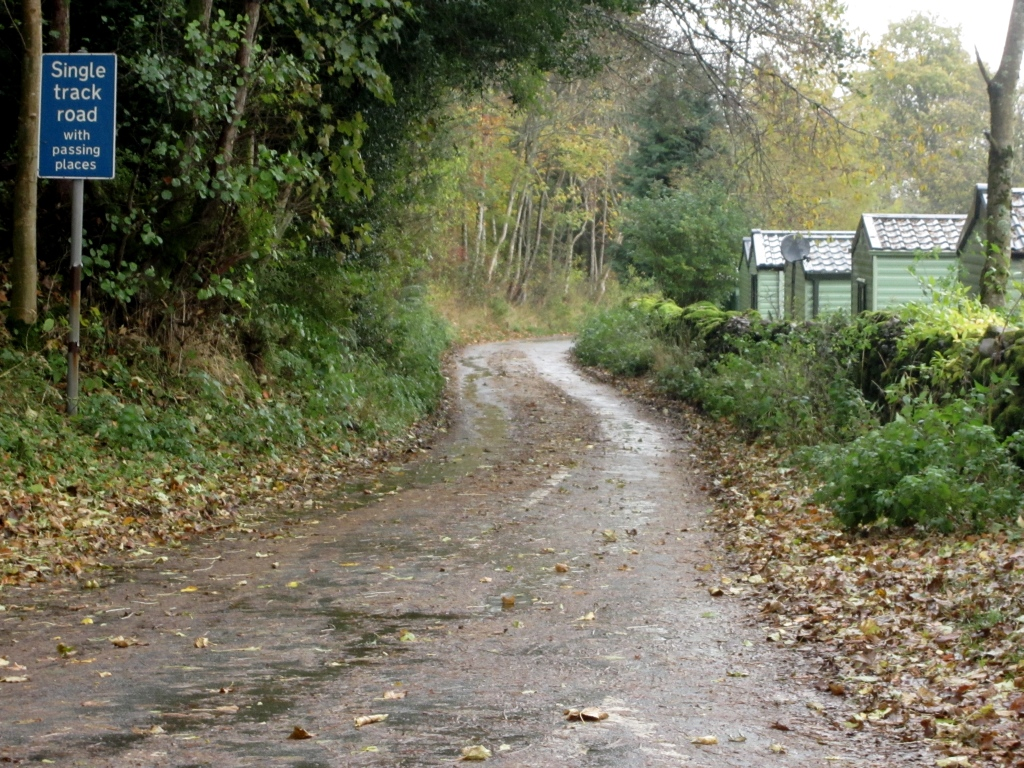
\includegraphics[width=0.488\textwidth,trim=0 65 0 12,clip]{Images/road_example.jpg}%
  }\hfill
  \subfloat[Single-lane warehouse rack corridor with AMR \cite{dematic_radial_amr}.]{%
    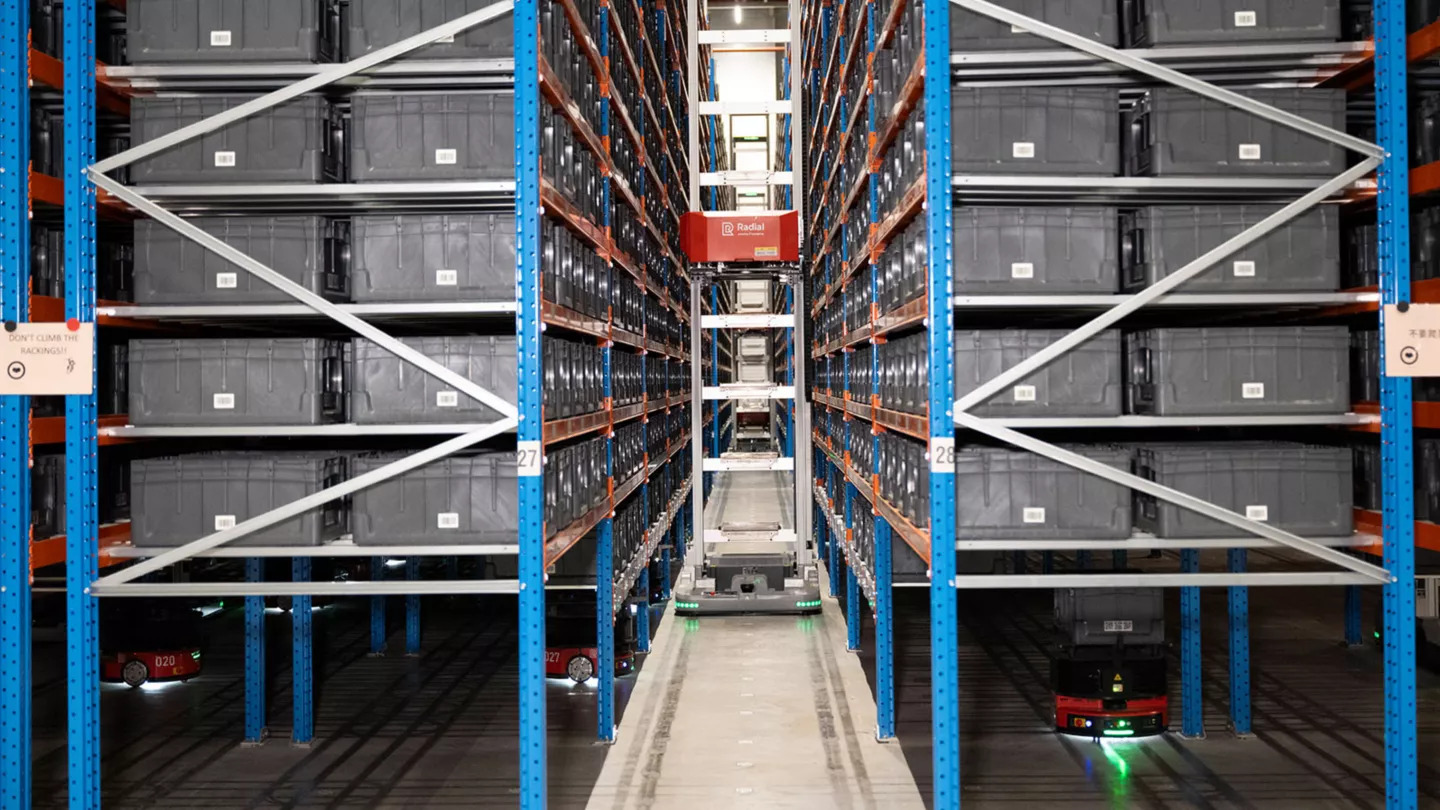
\includegraphics[width=0.488\textwidth]{Images/warehouse_example.jpg}%
  }
  \caption{Representative single-lane environments where two vehicles cannot pass side by side: (a) public road requiring discrete passing places, and (b) high-density warehouse with narrow aisles.}
  \label{fig:narrow_corridor_examples}
\end{figure*}

Given these limitations, an alternative approach is decentralized peer-to-peer negotiation. Rather than avoiding conflicts reactively or resolving them through a central authority (prescriptive collaboration \cite{george2025infrastructure}), encountering robots exchange compact messages over a local broadcast channel and agree on who yields and into which refuge. This retains the infrastructure-free operation of decentralized control while adding coordination to break symmetric deadlocks. 

Prior work spans fixed social laws and traffic rulebooks \cite{kato1992coordinating,shoham1995social,censi2019rulebooks}, market auctions \cite{gerkey2002sold,gautier2022negotiated}, incentive-compatible mechanisms for MAPF and robot prioritization \cite{amir2015mapfauction,das2021omcorp,friedrich2024scalable}, karma economies \cite{censi2019karma,elokda2024karma}, reinforcement-learned give-way policies \cite{bettini2022vmas,bettini2023heterogeneous,park2023hallucination}, and language-model negotiators \cite{marlin2024,gamechat2025,garg2024llm}. Despite this, three research gaps remain \cite{chandra2026social,francis2025principles}, as summarized below.

\begin{enumerate}
\item No shared refuge-and-reversing benchmark across policy families. Corridor give-way studies exist, including MARLIN's single- and two-slot corridors \cite{marlin2024}, VMAS \texttt{give\_way} \cite{vmasgiveway}, and narrow-hallway navigation \cite{park2023hallucination,alghamdi2025opinion}, but each evaluates one or two policy families. None compares rule-based, lock-based, market-based, mechanism-design, and learned policies on the same geometry with nonholonomic turn-and-park maneuvers, asymmetric reverse speeds, and multiple discrete bays (Table~\ref{tab:relwork}). Without such a testbed, competing policies cannot be compared fairly.

\item Siloed assumptions on information, incentives, and channels. Each community resolves conflicts under assumptions that ignore the others'. Rulebooks assume cooperative agents; auctions assume truthful cost estimates; mechanism-design studies assume lossless single-shot games; and communication-tolerant protocols rarely benchmark excess delay against a per-encounter hindsight reference. As a result, no single approach accounts for incentives, channel reliability, and delay together.

\item Unverified 2D-to-3D transfer. Fast 2D simulators make large statistical sweeps cheap but are rarely validated on a real stack. On hardware, wheel slip and acceleration limits alter motion, perception must infer the oncoming robot from noisy Lidar, and messages arrive with jitter rather than in lockstep. These delays are invisible in 2D, so yield decisions and excess-delay results that look sound there may stall or brake late under 3D physics and asynchronous timing.
\end{enumerate}

This paper addresses these gaps with a single refuge-and-reversing benchmark. The benchmark resolves the first gap directly, providing a common testbed that evaluates every policy under realistic turn-and-park maneuvers, asymmetric reverse speeds, and discrete bay placement. It also decomposes the second gap into three strands (information, incentives, and channels) and, for the third, tests which 2D results still hold on a real 3D stack. The study is organized around two architectural layers, namely, a decision mechanism layer determining who yields and into which refuge (RQ1--RQ2), and a distributed execution and embodiment layer governing how robots agree and execute under wireless loss, map errors, and 3D physics (RQ3--RQ4). Together, these layers frame four research questions, detailed next.

\begin{enumerate}
\item RQ1 (Information \& Cost Noise): How much delay do rulebooks, learned lookup tables, and kinematic cost bidding save over reactive backoff and corridor locking, and at what cost-estimation error do heuristic rules catch up to bidding?

\item RQ2 (Incentives \& Fairness): How easily can self-interested robots game unpriced or direct-transfer auctions, what are the budget and collusion trade-offs of Clarke-pivot payments, and how cheaply can historical delay credits balance repeated encounters?

\item RQ3 (Channel Loss \& Map Errors): How does periodic broadcast negotiation survive 99\% packet loss, which safeguards prevent collisions, and how can robots recover from incomplete or obstructed bay maps?

\item RQ4 (Multi-Robot Topologies \& 3D Transfer): What coordination primitives prevent deadlocks in 2-vs.-1 convoys and three-robot T-junctions, and where do 2D kinematic predictions diverge from 3D ROS~2/Gazebo execution?
\end{enumerate}

By addressing these research questions, this paper makes four main contributions.

\begin{enumerate}
\item Benchmark \& Dataset.
A modular ROS~2 benchmark is released that runs the identical 20\,Hz agent state machine in both a fast 2D simulator and 3D Gazebo Harmonic. Every 3D run is seed-paired to a 2D counterpart for direct one-to-one comparison across six narrow-corridor topologies (Fig.~\ref{fig:scen}).

\item Decision-Layer Characterization (RQ1--RQ2).
Reactive, reservation, rulebook, classifier, cost-bidding, and Clarke-pivot policies are benchmarked against the best yield choice across varying corridor geometries and robot speeds. This evaluation quantifies how policies degrade or hold up under log-normal bid noise ($\sigma\in[0,1]$), 27 strategic misreport profiles, and 20-encounter fairness sequences.

\item Protocol Ablation \& Map-Resilience Primitives (RQ3).
Three communication safeguards are ablated across 5,760 episodes under 90--99\% packet loss and 2--8\,s latency. The ablation records zero collisions in every configuration, even with all three radio safeguards disabled (indicating that local Lidar stopping margins and randomized exit timers, rather than the radio safeguards, prevent collisions), while the \texttt{commit} handshake adds 3--4\,s of waiting without reducing deadlocks. A zero-overhead map-recovery primitive piggybacks each robot's known bay list onto existing \texttt{BID} messages, restoring shared bay awareness under incomplete maps without extra packets.

\item Multi-Robot Extensions \& Gazebo Audit (RQ4).
Two-robot negotiation is extended to 2-vs.-1 convoys and three-robot T-junctions using follower backoff (\texttt{make\_room}), combined convoy bidding (\gb), and junction staging (\texttt{goal\_wait}), revealing why simply adding individual robot costs underestimates convoy yield time when the follower must reverse clear before the leader can back up. Across 496 seed-paired Gazebo runs, 2D and 3D select the same yielding robot in $97.0\%$ of encounters and match corridor excess delays within $1.0$~s, with the remaining differences traced to 3D Lidar detection range and three-robot junction timing.
\end{enumerate}

The remainder of this paper reviews related work (Sec.~\ref{sec:rel}), formulates the physical encounter and protocol architecture (Sec.~\ref{sec:bench}), defines the policy families and mechanism equations (Sec.~\ref{sec:pol}), details the experimental design and statistical conventions (Sec.~\ref{sec:exp}), presents empirical findings for RQ1--RQ4 (Secs.~\ref{sec:rq1}--\ref{sec:rq4}), synthesizes practitioner guidelines and limitations (Sec.~\ref{sec:disc}), and concludes (Sec.~\ref{sec:conc}).